\Aufgabe{Zwei Diagramme für eine Datenbank?}{
Folgende Diagramme stellen dieselbe Datenbank dar. 
Finde Unterschiede und erkläre wieso sie auftreten. Nutze bei Bedarf auch 
\UrlAndCode{www.dbiu.de/bayern/}

\vspace{0.3cm}

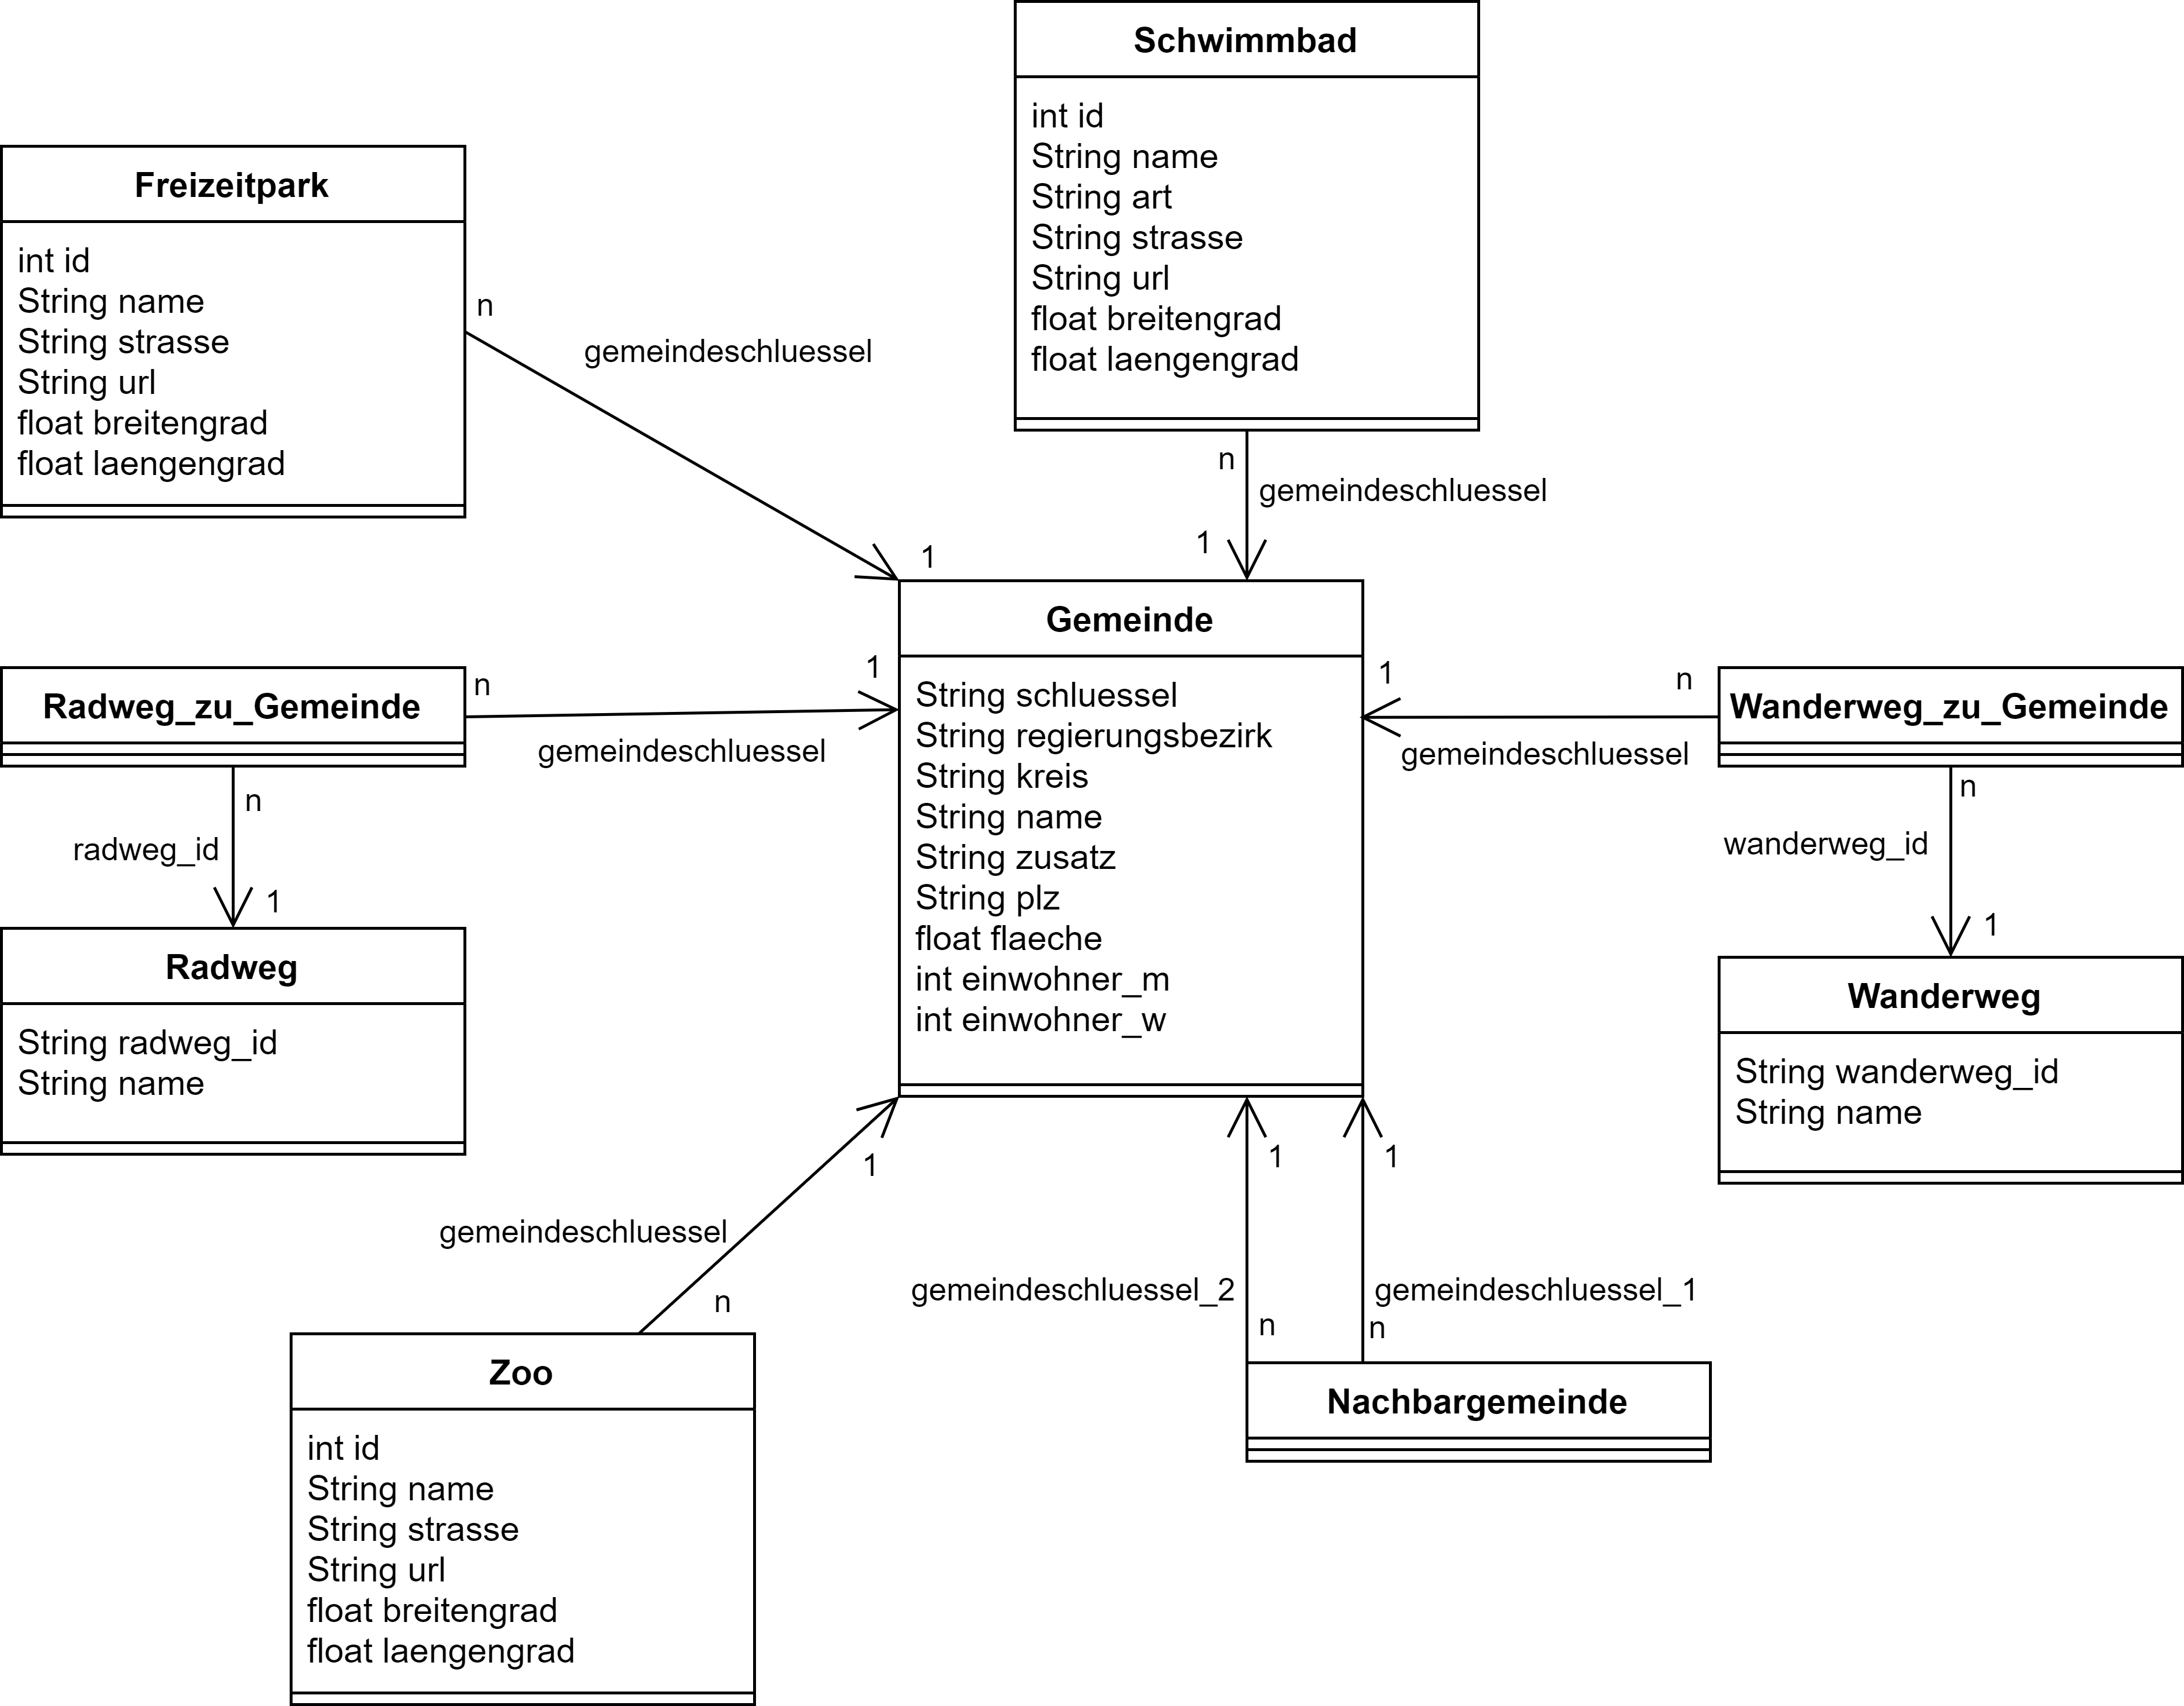
\includegraphics[width=0.92\textwidth]{_Aufgaben/img/A09_Bayern_DB.png}

\vspace{1cm}

\begin{tikzpicture}
    \begin{class}{Gemeinde}{0,0}
        \attribute{String schluessel}
        \attribute{String regierungsbezirk}
        \attribute{String kreis}
        \attribute{String name}
        \attribute{String zusatz}
        \attribute{String plz}
        \attribute{float flaeche}
        \attribute{int einwohner$\_$m}
        \attribute{int einwohner$\_$w}
    \end{class}
    \begin{class}{Freizeitpark}{-6.5,3}
        \attribute{int id}
        \attribute{String name}
        \attribute{String strasse}
        \attribute{String url}
        \attribute{float breitengrad}
        \attribute{float laengengrad}
    \end{class}
    \begin{class}{Schwimmbad}{6.5,3}
        \attribute{int id}
        \attribute{String name}
        \attribute{String art}
        \attribute{String strasse}
        \attribute{String url}
        \attribute{float breitengrad}
        \attribute{float laengengrad}
    \end{class}
    \begin{class}{Radweg}{0,3}
        \attribute{String radweg$\_$id}
        \attribute{String name}
    \end{class}
    \begin{class}{Wanderweg}{6.5,-4.2}
        \attribute{String wanderweg$\_$id}
        \attribute{String name}
    \end{class}
    \begin{class}{Zoo}{-6.5,-2.5}
        \attribute{int id}
        \attribute{String name}
        \attribute{String strasse}
        \attribute{String url}
        \attribute{float breitengrad}
        \attribute{float laengengrad}
    \end{class}
    
    \uniAssociationAngle
    {Freizeitpark.south}{270}
    {left}{n}
    {gemeindeschluessel}
    {1}{below}
    {180}{[shift={(0,1.5)}]Gemeinde.west}
    
    \uniAssociationAngle
    {Schwimmbad.south}{270}
    {right}{n}
    {gemeindeschluessel}
    {1}{below}
    {0}{[shift={(0,1.3)}]Gemeinde.east}
    
    
    \uniAssociationAngle
    {[shift={(0,0)}]Zoo.south east}{0}
    {right}{n}
    {gemeindeschluessel}
    {1}{below}
    {180}{[shift={(0,0)}]Gemeinde.south west}
    
    \biAssociationAngle
    {[shift={(2.5,0)}]Radweg.south}{270}
    {left}{n}
    {Radweg$\_$zu$\_$Gemeinde}
    {m}{left}
    {90}{[shift={(2,0)}]Gemeinde.north}
    
    \biAssociationAngle
    {[shift={(-1,0)}]Wanderweg.north}{90}
    {right}{n}
    {Wanderweg$\_$zu$\_$Gemeinde}
    {m}{above}
    {0}{[shift={(0,-1)}]Gemeinde.east}
    
    \biAssociationAngle
    {[shift={(1.7,0)}]Gemeinde.south}{270}
    {left}{n}
    {Nachbargemeinde}
    {m}{right}
    {270}{[shift={(-0.1,0)}]Gemeinde.south east}
\end{tikzpicture}

}